% !TEX program = xelatex -> bibtex -> xelatex*2

\documentclass[12pt]{ctexart}  
% ctexart支持中文编译文档
%最后全部翻译成英文后可以选择改成article,然后用pdflatex编译,还可以检验一下是不是没有中文了嘿嘿( •̀ ω •́ )✧
%官方要求字号不小于 12 号,此处选择 12 号字体

%\CTEXsetup[format={\Large\bfseries}]{section} 
\CTEXsetup[format={\Large\bfseries}]{section} 
%在ctexart中,一级标题是居中的,这里改成左对齐

%!!!
%文字包围图片

%% 本模板不需要填写年份,以当前电脑时间自动生成
%% !!!!!!!!!再研究一下ldmcm宏包
%% 请在以下的方括号中填写队伍控制号
\usepackage[2309397]{ldmcm}  % 载入ldmcm模板文件
\problem{C}  % 请在此处填写题号

%%字体选择
\usepackage{mathptmx}  % 这是 Times 字体,中规中矩
%!!!!! 
%\usepackage{mathpazo}  % 这是 COMAP 官方杂志采用的更好看的 Palatino 字体,可替代以上的 mathptmx 宏包

\usepackage{wallpaper}
\usepackage{colortbl}  %彩色表格需要加载的宏包
\usepackage{xcolor}
\usepackage{array}   %对表列和表格线的设置需要用到array宏包
\usepackage{enumitem}
\usepackage{fancyhdr}
\usepackage{wrapfig}
\usepackage{tcolorbox}
\usepackage{subfiles}
%%几处小修改,如无特殊需求可不做更改
\newcommand{\upcite}[1]{\textsuperscript{\textsuperscript{\cite{#1}}}}%这是参考文献引用上标的命令
\graphicspath{{img/}}          % 此处{img/}为相对路径,注意加上“/”
\let\itemize\compactitem
\let\enditemize\endcompactitem%解决列表环境中行距过大的问题

\title{Uncover the Hiddnd Secret in the Wordle Results}  % 标题

% 如需要修改题头(默认为 MCM /ICM),请使用以下命令(此处修改为 MCM)
%\renewcommand{\contest}{MCM}

% 设置行间距
\renewcommand{\baselinestretch}{1.0}
% ----------------------------------------------文档开始---------------------------------------------------------
\begin{document}
%!!!!!!
\setlength{\parindent}{0pt}

% 此处填写摘要内容-----------摘要摘要摘要摘要摘要摘要摘要摘要摘要摘要摘要摘要摘要摘要摘要摘要摘要摘要摘要摘要摘要
\begin{abstract}
	%第一段:2句话背景+2句话概括全文完成的任务
	%% !!有加粗
	%% Global warming, El Niño... With the emergence of various extreme climates,\textbf{Austral-ia's wildfires} occur more frequently. The greenhouse gases emitted after combustion have exacerbated global warming, which seems to have entered an endless loop. At the same time, hundreds of millions of lives have been killed in the fire, which makes us sad. To better control wildfires, we modeled the \textbf{distribution of drones} assisting in the observation to achieve the best balance between economy and efficiency.

	Since Wordle has become a popular puzzle game, it has accumulated a large amount ofdata. In this paper, we define a series of metrics and build several models to explore thehidden information in Wordle results.

	First, after \textbf{preprocessing} the given data and analyzing the time series diagram of thenumber of reported results, we found that the changes can be divided into 3 stages. Toforecast the number of reported results, we developed a weighted optimization modelbased on ARlMA and BP neural network. The prediction interval is then given usingthe Bootstrap method. We packaged this process as \textbf{ARIMA-BP Interval PredictionModel Based On Bootstrap}. Thus, we finally predicted the interval prediction valueobtained on March 1. 2023 at 95\% confidence level to be about (19504.74, 20383.26)

	Then, we defined 3 qualitative and 4 quantitative attributes of words and used them tobuild a \textbf{Multiple Linear Regression Model} with the percentage ofhard mode's playersWe found that the proportion will decrease by an average of0.618 when the initial letterchanges from a vowel to a consonant while it will increase by an average of0.017 foreach one-unit increase in word internal distance.

	After that, we made the percentage distribution prediction of the reported results basedon \textbf{LSTM Model}. To ensure the percentage is around 100\%, we first processed thecomponent data using a \textbf{spherical coordinate transformation}. Then we use them asoutput variables, the 7 word attributes and number ofresults as input to train our LSTMmodel. The prediction of EERlE based on this are [2\%,11\%, 25\%,24\%,19\%,14\%.5\%. We changed the model's parameters and added noise to do \textbf{sensitivity analysis}. Meanwhile, we introduced COV to measure the uncertainty of the model predictionand found that it is around 0.4. For \textbf{error analysis}, we use MSE, RMSE and R tomeasure the prediction accuracy, and their values are shown in Table 7.
	
	We extracted 6 indicators: RDC, TE, SK,NFC, NON, and HL to measure the dificultyof words. We built a \textbf{GMM Clustering Model} based on these indicators and thusclassifying 5 difficulty levels. We classified the word EERlE as dificulty level lll
	
	In addition, by counting the frequency of each letter in five positions, we found S as theinitial letter has the most frequency and more specific statistical results are shown inTable 9.We also used the \textbf{Association Rule Model} based on \textbf{Apriori algorithm} tomine the word combination pattern in Wordle, ldeally, we found that the letters A.S Eand F,TL usually appear together in Wordle.
	
	Finally, we evaluated and refined the model and reported the findings in a letter to thethe Puzzle Editor of the New York Times.
	
	\textbf{Keywords}: ARIMA-BP,LSTM, GMM, Apriori Algorithm, Word Attributes
	% %第二段:总结我们用了什么模型
	% Several models are established: Model I: Rasterized Multi-Objective Optimization Model; Model II: Model Verification Simulated by Poisson Process; Model III: Hovering Model Based on Tabu Search, etc.

	% %接下来分别介绍模型与结果
	% For Model I:
	% Firstly,%首先,我们从哪里收集到了什么样的数据
	% We find data。。。
	% Then,%然后,基于什么样的原因,我们建立了什么模型
	% we establish \textbf{model}。。。
	% Next,%我们选择或者设计了什么算法
	% we use Algorithm。。。
	% Finally,%我们得到了什么样的结果
	% %数值直接写出来,大量数据(表)或图片则说请参见(are shown in ...)图几
	% %注意要用文字,不要使用符号
	% it can be seen that。。。

	% For Model II:
	% Firstly,%首先,我们从哪里收集到了什么样的数据
	% We find data。。。
	% Then,%然后,基于什么样的原因,我们建立了什么模型
	% we establish model。。。
	% Next,%我们选择或者设计了什么算法
	% we use Algorithm。。。
	% Finally,%我们得到了什么样的结果
	% %数值直接写出来,大量数据(表)或图片则说请参见(are shown in ...)图几
	% %注意要用文字,不要使用符号
	% it can be seen that。。。

	% For Model III:
	% Firstly,%首先,我们从哪里收集到了什么样的数据
	% We find data。。。
	% Then,%然后,基于什么样的原因,我们建立了什么模型
	% we establish model。。。
	% Next,%我们选择或者设计了什么算法
	% we use Algorithm。。。
	% Finally,%我们得到了什么样的结果
	% %数值直接写出来,大量数据(表)或图片则说请参见(are shown in ...)图几
	% %注意要用文字,不要使用符号
	% it can be seen that。。。

	% %灵敏度与稳健性分析
	% Finally, sensitivity analysis 。。。 Meanwhile, robustness



	% 美赛论文中无需注明关键词。若一定要使用,
	% 请将以下两行的注释号 '%' 去除,以使其生效
	%\vspace{5pt}
	%\textbf{Keywords}: MATLAB, mathematics, LaTeX.

\end{abstract}

\maketitle  % 生成 Summary Sheet------------------------------------

\tableofcontents  % 生成目录


% -----------------------------------------正文开始-----------------------------------------------------------------------------------------------------------------------------------


%==============第一部分===引入=============================================================
\section{Introduction}
%!!!!!
%\subsection{Problem Background}%问题背景问题背景问题背景问题背景问题背景问题背景---------------------------------
\subsection{Background}
Wordle is an online word puzzle game invented by Josh Wardle during the epidemicThe New York Times newspaper which is well known for the games it publishes hasbought Wordle on February 2021\upcite{1}. Wordle only allows one game to be played perday, and every player in the world plays to guess the same five-letter word in six triesor less each day\upcite{2}. Players can play in regular mode or hard mode. They can sharetheir scores via Twitter, thus attracting more people to play and share
% 一些常用的写作缩略语:

% i.e.,。。。也即是。。。(一定加逗号)

% e.g.,。。。例如,。。。

% , etc.    。。。,等等。

% n.b.   特别注意

% cf.  参见


% 美赛一定要多上图,清晰直观,并且格式上最好是矢量图,例如pdf,而不是位图,例如jpg,png等,在形式上最好是组图,下面列出了利用\verb|subfigure|实现的
%!!!!
%\verb|1x2,1x3,2x2|的几种组图:

%% 这是一个1x2的组图
% \begin{minipage}[b]{0.4\linewidth}
% 	% \centering
% 	
\includegraphics[height=8\baselineskip]{img/example-image-a.pdf}
% 	\label{subfig:right}
% 	\caption{Wordle Game}
% \end{minipage}
% \begin{minipage}[b]{0.6\linewidth}
% 	Back in October 2021,less than 5.000 visitsregistered to its web page while by January 2022traffic had skyrocketed to over 45 million. Some ofus also love this game, Figure l shows one resulthat we got. The green tile indicates that the secretsolution word has the letter in the precise locationThe yellow tile implies that the answer has theletter but not at the correct location. Grey tilesindicate the letters are not contained in the solutionat all\upcite{3}.
% \end{minipage}
\begin{wrapfigure}{l}{6cm}
	\vspace{-15pt}
	\includegraphics*[width=0.4\textwidth]{example-image-a.pdf}
	\vspace{0pt}
	\caption{Wordle Game}
	\vspace{-20pt}
\end{wrapfigure}
Back in October 2021,less than 5.000 visits registered to its web page while by January 2022traffic had skyrocketed to over 45 million. Some ofus also love this game, Figure l shows one resulthat we got. The green tile indicates that the secretsolution word has the letter in the precise locationThe yellow tile implies that the answer has theletter but not at the correct location. Grey tilesindicate the letters are not contained in the solutionat all\upcite{3}.

	% \hspace{10mm} %%%%%%%%%%%%%%%%%%调整子图间距
	% \begin{subfigure}[b]{.3\textwidth}
	% 	\includegraphics[width=\textwidth]{img/example-image-b.pdf}
	% 	\caption{right}\label{subfig:right}
	% \end{subfigure}
	% \label{subfigure}

%Figure gives an example of subfigures. Figure \ref{subfig:left} is on the left, and Figure is on the right.
Now we have a file of daily results from January 7, 2022 to December 31, 2022. Thisfile includes twelve key variables that are crucial in our later research. In the file, the percentages of the number of people for the seven tries may not sum to 100\% due to rounding

% %% 这是一个1x3的组图
% \begin{figure}[!htbp]
% 	\centering
% 	\begin{subfigure}[t]{0.3\textwidth}
% 		\centering
% 		
\includegraphics[width=\textwidth]{img/example-image-a.pdf}
% 		\caption*{}
% 		\label{}
% 	\end{subfigure}
% 	\begin{subfigure}[t]{0.3\textwidth}
% 		\centering
% 		\includegraphics[width=\textwidth]{img/example-image-b.pdf}
% 		\caption*{}
% 		\label{}
% 	\end{subfigure}
% 	\begin{subfigure}[t]{0.3\textwidth}
% 		\centering
% 		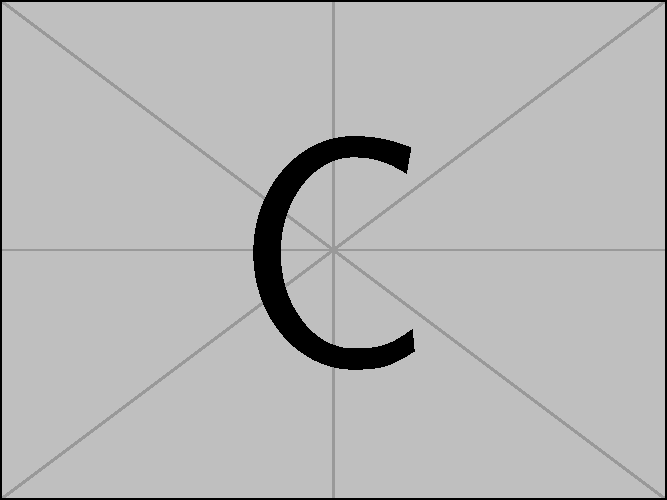
\includegraphics[width=\textwidth]{img/example-image-c.pdf}
% 		\caption*{}
% 		\label{}
% 	\end{subfigure}
% 	\caption{Three images}
% 	\label{Three images}
% \end{figure}


% %% 这是一个2x2的组图(可推广至2x3,3x3等)
% \begin{figure}[!htbp]
% 	\centering
% 	\begin{subfigure}[t]{0.4\textwidth}
% 		\centering
% 		
\includegraphics[width=\textwidth]{img/example-image-a.pdf}
% 		\caption{左上}
% 		\label{}
% 	\end{subfigure}
% 	\begin{subfigure}[t]{0.4\textwidth}
% 		\centering
% 		\includegraphics[width=\textwidth]{img/example-image-b.pdf}
% 		\caption{右上}
% 		\label{}
% 	\end{subfigure}
% 	%  \begin{subfigure}[t]{0.3\textwidth}
% 	%          \centering
% 	%          
\includegraphics[width=\textwidth]{img/example-image-a.pdf.pdf}
% 	%          \caption{}
% 	%          \label{}
% 	%  \end{subfigure}
% 	\qquad
% 	%%让图片换行,这就是实现多行组图的简单原理
%   %%若需要搞一个2x3的组图就把上下的注释打开再添加图片就可以了
%   %%注意调整比例以及间距
% 	\begin{subfigure}[t]{0.4\textwidth}
% 		\centering
% 		
\includegraphics[width=\textwidth]{img/example-image-a.pdf}
% 		\caption{左下}
% 		\label{}
% 	\end{subfigure}
% 	\begin{subfigure}[t]{0.4\textwidth}
% 		\centering
% 		\includegraphics[width=\textwidth]{img/example-image-b.pdf}
% 		\caption{右下}
% 		\label{}
% 	\end{subfigure}
% 	%\begin{subfigure}[t]{0.3\textwidth}
% 	%        \centering
% 	%        \includegraphics[width=\textwidth]{img/npca13.pdf}
% 	%        \caption{result}
% 	%        \label{}
% 	%\end{subfigure}
% 	\caption{组图组图变变变}
% \end{figure}



%\subsection{Problem Background}%问题重述与文献综述选一个------------------------------------------------------------------------
\subsection{Problem Restatement} % 文献综述-----------------
By analyzing the above background, we summarize the tasks that need to be addressedas follows:
\begin{itemize}
	\item Develop a model to explain the daily variation in the total number of peoplereporting scores on Twitter and use it to give a prediction interval for the totanumber of people on March 1.2023.
	\item Determine whether the attributes of words affect the percentage of playerswho choose the hard mode and explain the obtained results accordingly.
	\item If given a future date and the specific word, build a model to predict thepercentage of 1-X tries in this day. After that, the word EERlE on March 1. 2023should be used as a specific example of the model prediction, while analyzing theuncertainties of the model and the accuracy of the prediction.
	\item Develop a model to classify the diffculty of the words and identify theattributes of them under each category. Use this model to determine how difficultthe word EERlE is? Finally, discuss the accuracy ofthe classification model
	\item List and describe some other interesting features of the dataset
\end{itemize}
% A literatrue\upcite{1} says something about this problem ...



\subsection{Our work}%-----------------------------------------------------------
\begin{figure}[htbp]
	\centering
	\includegraphics[height=8\baselineskip]{example-image-b.pdf}
	\caption{Our Work}
	\vspace{-20pt}
\end{figure}

\section{Assumptions and Notations}
\vspace{0pt}
%为了简化问题,我们做出了以下假设,其中每一条都有对应的合理解释
% \begin{itemize}
% 	\item \textit{\textbf{Assumption 1:}}假设\\$\hookrightarrow$ \textit{\textbf{Explanation:}}理由

% 	\item \textit{\textbf{Assumption 2:}}假设\\$\hookrightarrow$ \textit{\textbf{Explanation:}}理由

% 	\item \textit{\textbf{Assumption 3:}}假设\\$\hookrightarrow$ \textit{\textbf{Explanation:}}理由

% 	\item \textit{\textbf{Assumption 4:}}假设\\$\hookrightarrow$ \textit{\textbf{Explanation:}}理由
% \end{itemize}
\textbf{Assumption 1:}The number of daily online gamers in the data set is a time-dependentset of series and is independent of seasonal changes.
\\
\textbf{Explanation:} Therefore, we can use ARlMA as well as LSTM models to predict a series ofdata for March 1.2023.
\\
\\
\textbf{Assumption 2:}The scores reported by players on Twitter on a daily basis are normaland reliable.
\\
\textbf{Explanation:}To ensure that the model we build based on the dataset can reliably predict arange of data for March 1.2023.
\\
\\
\textbf{Assumption 3:}Assuming that Wordle's development process is consistent with thegame's life cycle theory.
\\
\textbf{Explanation:} This assumption reduces the impact ofexternal uncertainties on Wordle gamepredictions, thus making the whole process of prediction and analysis more efficient.

%这里只列出了主要的假设,其他假设会在专门的小节中单独讨论
In this work, we use the symbols in Table 1 in the model construction. Other none-frequent-used symbols will be introduced once they are used.

%\subsection{Notations}%-----------------------------------------------------------------------------------
% % 三线表(可以直接在excel里编辑好然后用excel2latex插件插入)

%Table \centering\small\ref{tb:notation} %lists some important mathematical notations used in this paper.

\begin{table}[htbp]%----------------------------------------------
	\renewcommand{\arraystretch}{1.1}
	\begin{center}
		\caption{Notations}
		\centering
		\begin{tabular}{cl}
			\toprule[1.5pt]
			\multicolumn{1}{m{4cm}}{\centering \textbf{Symbol}}
			                      & \multicolumn{1}{m{10cm}}{\centering \textbf{Defination} }                       \\
			\midrule
			$w_A$                 & Longitude within the i-th Wildfire Grid                                \\
			$w_B$                 & Latitude within the i-th Wildfire Grid                                 \\
			$P_{Ai}$              & The area of the i-th grid                                              \\
			$P_{Ai}$              & the distance $d_{ki}$                                                  \\
			$L_i$                 & Score for evaluating the k-th wildfire grid                            \\
			%\vspace{5pt}%公式间有点挤,空一些
			%$x^{( \alpha )}_{ki}$ & the $SSA_\alpha$ drone sent by the k-th EOC to the i-th wild-fire grid \\
			$NF$                  & Noise factor                                                           \\
			$C_i$                 & the ratio of players at different guess counts                         \\
			% \vspace{3pt}
			%$x^{( \beta )}_{ki}$  & the $RR_\beta$ drone sent by the k-th EOC to the i-th wildfire grid    \\
			%$t_{fly}^{\delta}$    & The flight time of drones                                              \\
			\bottomrule[1.5pt]
		\end{tabular}
		\label{tb:notation}
		% \begin{tablenotes}
		% 	\footnotesize
		% 	\item[*] *Some variables are not listed here and will be discussed in detail in each section. %此处加入注释*信息
		% \end{tablenotes}
	\end{center}
\end{table}
\vspace{-1cm}
%在\end{table}下加一行\vspace{-1cm} 其中-1的作用是缩短与下方文字距离的 切记!必须是负数



%数据处理------------------------------------------------------------------------

\newpage
\section{ARIMA-BP Interval Prediction Model Based On Bootstrap}
\subsection{Data Processing}
%下面列出了我们收集数据的来源网站
By reviewing the given data, we found that there are no missing values, but there areive outliers, One of them does not exist and two of them has less than 5 letters. wedeleted these three rows of data due to the difficulty ofobtaining the true values ofthesewords. The two remaining outliers are caused by data entry errors. In order to avoid anexcessive reduction in the amount of data, we changed them by combining the previousand later data as well as the semantics ofthem, In addition, the sum of the percentagesin the original data are all in [98\%, 102\%], which is not much different from 100\%, sothey are reasonable and do not need to be processed. In summary, the preprocessing ofthe raw data is summarized in Table \ref{tb:data}.

\begin{table}[htbp]%----------------------------------------------
	\begin{center}
		\caption{Data Processing}
		\begin{tabular}{c c c c}
			\toprule[1.5pt]
			\multicolumn{1}{m{5cm}}{\centering \textbf{Database Names}}
			               & \multicolumn{1}{m{10cm}}{\centering \textbf{Database Websites}}   \\
			\midrule
			Google Scholar & \href{https://scholar.google.com} {https://scholar.google.com}    \\
			Wikipedia      & \href{https://www.wikipedia.org}{https://www.wikipedia.org}       \\
			wolframalpha   & \href{https://www.wolframalpha.com}{https://www.wolframalpha.com} \\
			\bottomrule[1.5pt]
		\end{tabular}
		\label{tb:data}
	\end{center}
\end{table}
\vspace{-1cm}%在\end{table}下加一行\vspace{-1cm} 其中-1的作用是缩短与下方文字距离的 切记!必须是负数

\subsection{Point Prediction Based on a Combined ARIMA-BP Model}
%=================================第三部分====================================================================
\subsubsection{Variation Explaining}
In the data preprocessing, although there are word entry errors, their correspondingnumbers of reported results are not aflected, so the complete reported data are analyzedin this problem. By observing and analyzing the characteristics of the changes in thenumber of reported results from Jan.7, 2022 to Dec 31, 2022, we found that they canbe divided into 3 phases, as shown in Figure 3.
\\
Based on the game lifecycle and player lifecycle theory[4], and combined with Wordle'sgame features, we explain the reasons for the changes as follows.

% \noindent
% \begin{itemize}{\leftmargin=0pt\setlength{\parindent}{0pt}}
% 	\item {Phase 1:} 
% 	\\Rapid Growth Period (January 7\, 2022-February 2\, 2022)
% \end{itemize}

\raisebox{-0.8ex}{\scalebox{2.2}{\textbullet}}\hspace{0.5em} Phase 1: Rapid Growth Period (January 7\, 2022-February 2\, 2022)

Since the launch of Wordle's web version, it has been updated with only one puzzle aday. This artificial scarcity enhances players' desire for challenge and anticipation. Thesharing function of Wordle uses emoji blocks to refer to the results of the game, whichis very recognizable and easy to spread, while also avoiding spoilers, thus attractingmore new players to play Wordle. In addition, the traditional popularity of crosswordpuzzles and the easy-to-play game mechanics have contributed to Wordle's furtheipopularity. During this period, Wordle's overall growth in the number ofresults reportedis 348.85\%, with the number peaking at 361.908 on February 2.

% \begin{equation}\label{eq:heat}
% 	\frac{\partial u}{\partial t} - a^2 \left( \frac{\partial^2 u}{\partial x^2} + \frac{\partial^2 u}{\partial y^2} + \frac{\partial^2 u}{\partial z^2} \right) = f(x, y, z, t)
% \end{equation}

\begin{figure}[htbp]
	\centering
	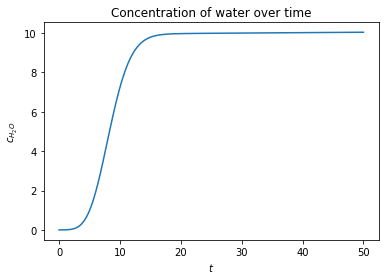
\includegraphics[height=9\baselineskip]{water.png}
	\caption{Changes in the number of reported results}
\end{figure}

\raisebox{-0.8ex}{\scalebox{2.2}{\textbullet}}\hspace{0.5em} Parse 2: Rapid Decline Period (February 3, 2022 - May 29,2022)
During this period, Wordle experiences an overall 84.29\% decline in the number ofreported results, which is the general nature of internet fads. When the popularity ofthegame reaches its peak, it faces a significant loss of players due to gamers’declininginterest and boredom with the game. The singularity of Wordle's game mechanic cancontribute to this. Furthermore, the emergence of competing games in the market suchas “Words with Friends’ and Wordle's pirated games makes Wordle lose players further
% \section{Model 2}
% \subsection{Conclusion of Model 2}
% The results are shown in Figure \ref{fig:result}, where $t$ denotes the time in seconds, and $c$ refers to the concentration of water in the boiler.

% \begin{figure}[!ht]%---------------结果上图!!!!!!--------------
% 	\centering
% 	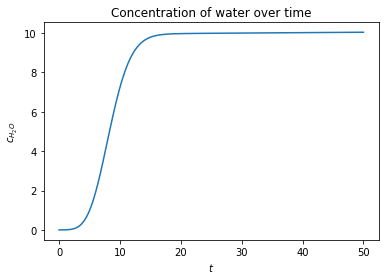
\includegraphics[width=.5\textwidth]{water.png}
% 	\caption{The result of Model 2}\label{fig:result}
% \end{figure}%---------------------------------------------

%!!!!!!伪代码
% 再来一个伪代码,默认样式为\texttt{隐藏行号的三线表形式的伪代码}

% 可在\verb|ldmcm.sty|中修改样式,更详细的用法请参考algorithm2e宏包文档
% %%%%%%%%%%伪代码%%%%%%%%%%%%%%%%%%%%%%

% \begin{algorithm}[H]
% 	\KwIn{输入}
% 	\KwOut{输出 }
% 	initialization\;
% 	\While{not at end of this document}{
% 		read current\;
% 		\Repeat{this end condition}{
% 			do these things\;
% 		}
% 		\eIf{understand}{
% 			go to next section\;
% 			current section becomes this one\;
% 		}{
% 			go back to the beginning of current section\;
% 		}
% 		\Do{this end condition}{
% 			do these things\;
% 		}
% 	}
% 	\caption{How to write algorithms}
% \end{algorithm}
% %%%%%%%%%%伪代码%%%%%%%%%%%%%%%%%%%%%%

\raisebox{-0.8ex}{\scalebox{2.2}{\textbullet}}\hspace{0.5em} Parse 3: Stable Reduction Period (May 30,2022-December 31,2022)
The overall decrease in the number of results reported for Wordle in this phase is 64.14\%. Rapidly losing players in Phase 2 go to play Wordle generally because of itspopularity among the general public and they will quickly leave when Wordle is nolonger hot or the next trend emerges. The remaining players are often loyal Wordleplayers or players who have developed user stickiness due to the game's social circleAt this point, the number of reports will still drop but not by much.


\subsubsection{Reasons for Model Selection}
Predicting the number of reported results is a problem in the field oftime series analysisThe traditional ARlMA model is capable of extracting deterministic information fromhistorical data in order to predict the trend of variables over time, however, this moderequires extensive testing before application, and the process of determining the orderofthe model is subjective to some extent [5]. In recent years, with the development ofartificial intelligence, machine learning algorithms have been widely applied to the fieldof data classification and prediction. Among which, BP neural network model which iseficient and convenient can effectively break the limits of traditional time seriesprediction models. Considering these factors, we decide to combine the advantages oftraditional time series models and machine learning models. It means that first of all.we use ARlMA model and BP neural network model to predict the number of reportedoutcomes separately, and then we use weighted average to combine the two models toobtain a more reliable ARlMA-BP combined prediction model.

%The instance of long and wide tables are shown in Table \ref{tb:longtable}.

% 长表格示例,更多用法请参考 longtable 宏包文档
% 以下环境及对应参数可实现表格内的自动换行与表格的自动断页
% 您也可以选择自行载入 tabularx 宏包,并通过 X 参数指定对应列自动换行
% \begin{longtable}{ p{4em} p{14em} p{14em} }
% 	\caption{Basic Information about Three Main Continents (scratched from Wikipedia)}
% 	\label{tb:longtable}                                                                                                                      \\
% 	\toprule
% 	Continent                                                  & Description                                                    & Information \\
% 	\midrule
% 	Africa                                                     & Africa Continent is surrounded by the Mediterranean Sea to the
% 	north, the Isthmus of Suez and the Red Sea to the northeast, the Indian
% 	Ocean to the southeast and the Atlantic Ocean to the west. &
% 	At about 30.3 million km$^2$ including adjacent islands, it covers 6\%
% 	of Earth's total surface area and 20\% of its land area. With 1.3
% 	billion people as of 2018, it accounts for about 16\% of the world's
% 	human population.                                                                                                                         \\
% 	\midrule
% 	Asia                                                       & Asia is Earth's largest and most populous continent which
% 	located primarily in the Eastern and Northern Hemispheres.
% 	It shares the continental landmass of Eurasia with the continent
% 	of Europe and the continental landmass of Afro-Eurasia with both
% 	Europe and Africa.                                         &
% 	Asia covers an area of 44,579,000 square kilometres, about 30\%
% 	of Earth's total land area and 8.7\% of the Earth's total surface
% 	area. Its 4.5 billion people (as of June 2019) constitute roughly
% 	60\% of the world's population.                                                                                                           \\
% 	\midrule
% 	Europe                                                     & Europe is a continent located entirely in the Northern
% 	Hemisphere and mostly in the Eastern Hemisphere. It comprises the
% 	westernmost part of Eurasia and is bordered by the Arctic Ocean to
% 	the north, the Atlantic Ocean to the west, the Mediterranean Sea to
% 	the south, and Asia to the east.                           &
% 	Europe covers about 10,180,000 km$^2$, or 2\% of the Earth's surface
% 	(6.8\% of land area), making it the second-smallest
% 	continent. Europe had a total population of about 741 million (about
% 	11\% of the world population) as of 2018.                                                                                                 \\
% 	\bottomrule
% \end{longtable}

\subsubsection{ARIMA Forecasting}
We first used the traditional ARlMA model for point prediction of the number ofreported results, and this process is shown in Figure \ref{fg:process}:
\begin{figure}[htbp]
	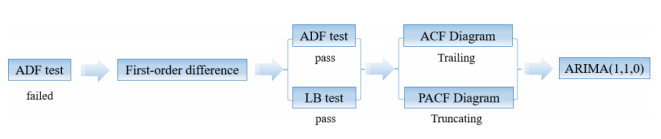
\includegraphics[width=\textwidth]{1706015643684.png}
	\caption{ARIMA model building process}
	\label{fg:process}
\end{figure}

First, we performed ADF smoothness test on the variable “Number ofreported resultsin the preprocessed data set and found that it wasn't smooth. Therefore, we differencedthe series to the first order and tested the diferenced series again. After that, weobserved the ACF and PACF plot of the differenced series, and found that the ACF plotshowed the characteristics of trailing tails and the PACF plot showed the characteristicsof lst order truncated tails. Therefore, the following ARIMA(1.1.0) model can bedeveloped for the original series:

\begin{equation*}
	\centering
	\begin{cases}
		(1-\phi_1B)(1-B)x_t=\varepsilon_t\\
		E(\varepsilon_t)=0,Var(\varepsilon_t)={\sigma_{\varepsilon}}^2,E(\varepsilon_t\varepsilon_s)=0,s\neq t,\\
		E(x_s\varepsilon_t)=\mathbf{0},\forall s<t
	\end{cases}
\end{equation*}
where $x_t$ is the $t^th$ time series value, $B$ is the delay operator, $\phi_1$ is the coeffcient of the moving self-averaging polynomial.

\subsubsection{BP Neural Network Prediction}
BP neural network is a multilayer feedforward neural network trained according to theerror back propagation algorithm, which can iterate and repair its own weightscontinuously based on the relationship between input and output variables so as tofinally estimate the exact functional relationship\upcite{6}. Its algorithm is explained by thefollowing pseudo-code. :


% \begin{algorithm}[H]
% 	\KwIn{Training set D}
% 	\KwOut{test set E}{
% 		% initialization\;
% 		\hspace{1.5em}\begin{tabular}{|l}
% 			Learning rate ŋ;Data normalization(normalization formula)\\
% 			Create network;Train the network
% 		\end{tabular}
		
% 		\hspace{1.5em}\begin{tabular}{|l}
% 			\hspace{2em}\begin{tabular}{|l}
% 				repeat for D\\
% 				Forward propagation;Backward propagation\\
% 				until for reaches end condition
% 			\end{tabular}\\
% 			Using the network;Inverse normalization of data\\
% 			BP neural network prediction with test set E
% 		\end{tabular}
		
% 	\textbf{end:}The completed BP neural network trained}
% \end{algorithm}

\begin{algorithm}[H]
	\KwIn{Training set $D$}
	\KwOut{Test set $E$}{
		\hspace{1.5em}\begin{tabular}{|l}
		Learning rate $\eta$;Data normalization (normalization formula)\\
		Create network; Train the network\\
	    \end{tabular}

		\hspace{1.5em}\begin{tabular}{|l}
			\hspace{2em}\begin{tabular}{|l}
			repeat for D\\
			Forward propagation; Backward propagation\\
			until for reaches end condition
		\end{tabular}\\
		Using the network; Inverse normalization of data\\
		BP neural network prediction with test set E
	\end{tabular}\\
	\textbf{end:}The completed BP neural network trained}
	\caption{Prediction of the Number of Reported Results}
\end{algorithm}

%===============================================第四部分=============================================
\subsubsection{Analysis of the Results}
The result obtained using the ARlMA(1,1,0) model prediction is shown in Figure \ref{fg:5}.and using the BP neural network model prediction is shown in Figure \ref{fg:6}:
\begin{figure}[!htbp]
	\centering
	\begin{subfigure}[t]{0.4\textwidth}
		\centering
		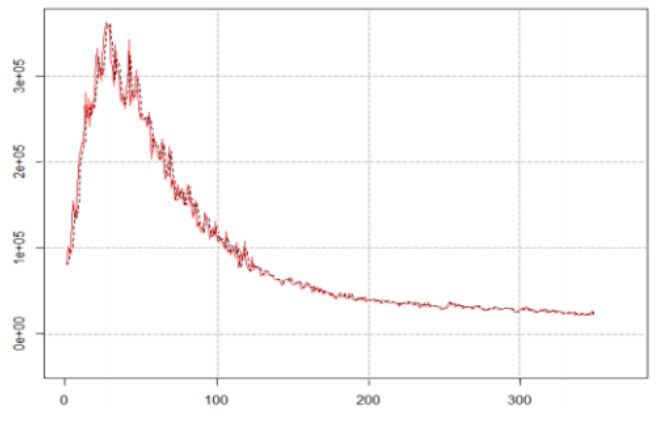
\includegraphics[width=\textwidth]{1706018588496.png}
		\caption{ARIMA prediction effect}
		\label{fg:5}
	\end{subfigure}
	\begin{subfigure}[t]{0.4\textwidth}
		\centering
		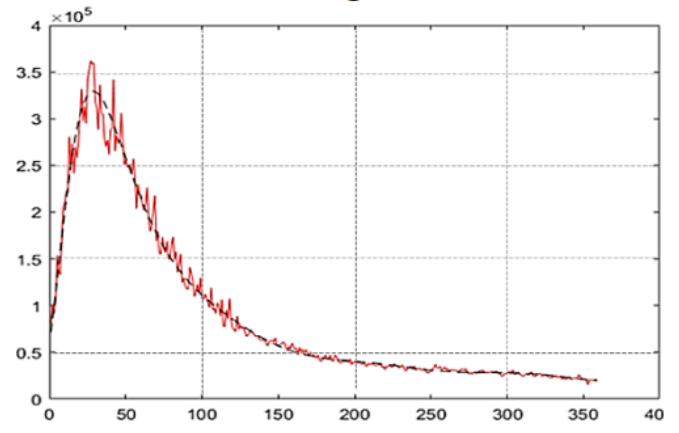
\includegraphics[width=\textwidth]{1706018630565.png}
		\caption{BP neural network prediction effect}
		\label{fg:6}
	\end{subfigure}
	\caption{Three images}
	\label{Three images}
\end{figure}

It can be seen that the ARlMA model has a better effect prediction, and the pointprediction Pa obtained using this model for the number of results reported on March 1.2023 is about 20598.84. BP neural network model has some bias in the early stage buthas relatively good prediction effect in the later stage. The point prediction value Peobtained using this model on March 1, 2023 is about 19496.05.

\subsubsection{Weighted Portfolio Model Forecast}
In order to improve the accuracy and robustness of the model prediction, we derived anew combined ARlMA-BP prediction model based on ARlMA and BP neural networkmodel by using the prediction errors to weight the two models. The design idea of thisweighted combined forecasting model is shown in Figure \ref{fg:7}:
\begin{figure}[htbp]
	\centering
	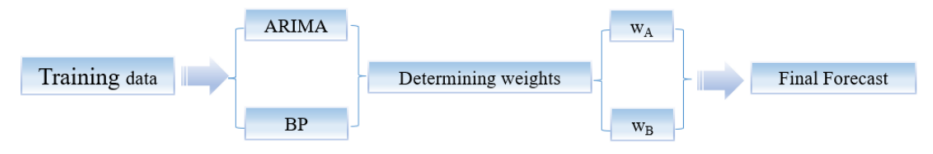
\includegraphics[width=\textwidth]{1706018870335.png}
	\caption{Combined model design}
	\label{fg:7}
\end{figure}
We first calculate the average prediction error for each of the two prediction models:
\begin{equation*}
	\overline{PEA^2}=\frac{1}{N}\sum_{i=1}^{N}(R_i-P_{Ai})^2,\overline{PEB^2}=\frac{1}{N}\sum_{i=1}^{N}(R_i-P_{Bi})^2.
\end{equation*}
%!!!!overline{}, frac{}{}, \sum{i=1}^{N},
After that, we use the share of the average prediction error squared of either model inthe total average prediction error squared of the two models to reflect the weightaccounted for by the other model, i.e.
%!!!i.e
\begin{equation*}
	w_A=\frac{\overline{PEB}^2}{\overline{PEA}^2+\overline{PEB}^2}\approx0.406,  w_B=\frac{\overline{PEA}^2}{\overline{PEA}^2+\overline{PEB}^2}\approx0.594
\end{equation*} 
Thus, the point prediction value of the $i^th$series in the final ARIMA-BP combination model obtained is calculated as:
\begin{equation}
	P_i=w_{A}P_{Ai}+w_{B}P_{Bi}\label{eq:1}
\end{equation}

\newpage
Through the analysis of the prediction errors above, it is obvious that the overalprediction error ofARlMA model is relatively high, while the BP neural network modelmay be overfitted. Therefore, the combined ARlMA-BP prediction model can correctthe errors of these two models, thus making the prediction results more realistic.
\begin{figure}[htbp]
	\centering
	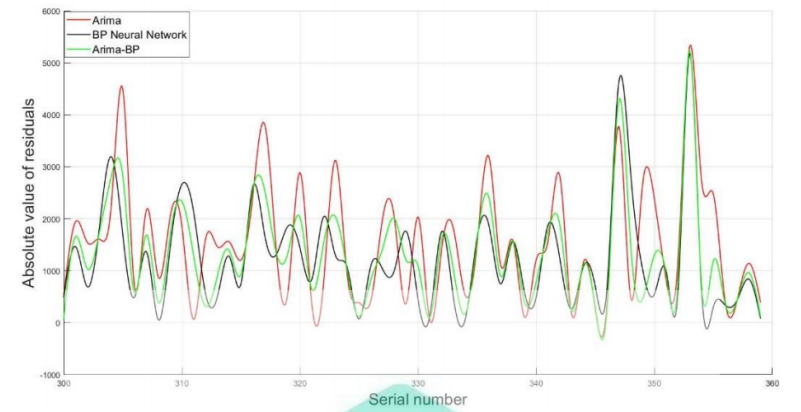
\includegraphics[width=\textwidth]{1706020552100.png}
	\caption{Prediction errors of the three models}
	\label{fg:8}
\end{figure}
The final point forecast for the number of results reported on March 1, 2023 using thiscombined ARIMA-BP model is approximately 19944.

\subsection{Interval Prediction Based on Bootstrap Model}
Bootstrap Method
%!!!!set[9]
The Bootstrap method is an important method used in statistics for interval prediction,which first assumes that the data set obeys an unknown distribution, and later estimatesthe distribution interval of the sample by repeatedly sampling the given data set [7].Wetook the data predicted under the weighted combination model for the next 60 periodsas the sample set, after which we sampled it 1000 times with put-back to obtain the1000 Bootstrap sample set, $y_B$=($Y$,$Y_2$,\textbullet\textbullet\textbullet\textbullet\textbullet\textbullet, $Y_1000$).
\\
For each subsample, the distribution is in line with that ofthe sample, so we calculatedthe standard deviation (SD) ofthese 1000 subsample sets as the SD ofthe sample:

\begin{equation*}
	\sqrt{Var(y)}=\sqrt{\frac{1}{N-1}\sum_{i=1}^{N}(y_i-\overline{y})^2}
\end{equation*}
According to the central limit theorem, it is known that the set of samples obtained byconducting 1000 draws approximately obeys the normal distribution. Therefore, the upper and lower limits ofthe confidence interval of the sample at confidence level 1-$\alpha$ be calculated with the help of z-statistic:
\begin{equation}
	y=\stackrel{\wedge}{y}\pm Z_{\alpha/2}\times\sqrt{Var(y)}.\label{eq:2}
\end{equation}
Taking the confidence levels of 95\%, 90\% and 80\% respectively, the final prediction intervals for the number of results reported on March 1, 2023 are shown in Table \ref{tab:addlabel}
% Table generated by Excel2LaTeX from sheet 'Sheet1'

%!!!!!颜色
\begin{table}[htbp]
    \centering  % 居中
    \caption{Confidence Intervals}
	\arrayrulecolor{blue}
	\setlength{\tabcolsep}{0.09\textwidth}{
    \begin{tabular}{|c|c|c|}
		\arrayrulecolor{blue}\hline
        \textbf{Confidence level} & \textbf{Lower limit} & \textbf{Upper limit} \\
        \arrayrulecolor{blue}\hline
		\rowcolor{blue!20}95\% & 19504.74 & 20383.26 \\
		\arrayrulecolor{blue}\hline
        90\% & 19575.33 & 20312.67 \\
		\arrayrulecolor{blue}\hline
        \rowcolor{blue!20}80\% & 19656.69 & 20231.31 \\
		\arrayrulecolor{blue}\hline
    \end{tabular}}
    \label{tab:addlabel}
\end{table}

\section{Exploring the Impact of Word Attributes on Hard Mode Based on Multiple Linear Regression Model}

Exploring the effects of certain attributes of words on the proportion of playerschoosing Hard Mode is a multiple-input variable, single-output variable modelingproblem. We decided to develop a multiple linear regression model to derive whetherword attributes affect the percentage of scores reported that were played in Hard Modeand the extent oftheir effects. The input variables X1-X7 are defined as follows.
\subsection{Defining Qualitative Attributes of Words}
First we made an overview of all the words in the dataset, and drew a word cloud mapfor the 356 words after preprocessing in Figure 9. We found that each word is differentand its frequency is l, so its size in the word cloud map is about the same.
\subsection{Defining Quatitative Attributes of Words}
\begin{equation}
	WID_n=\sum_{i=1}^{4}|L_{i+1}-L_i|, n=1,2,3,\cdots,357
\end{equation}

\subsection{Building a Multiple Linear Regression Model}

\begin{equation*}
	\centering
	X_1=\begin{cases}1, noun\\2, verb\\3, adjective\\4, other\end{cases}, X_2=\begin{cases}1, commom\\2, uncommom\end{cases}, X_3=\begin{cases}1, vowel\\2, consonant\end{cases}
\end{equation*}
The dependent variable (Y) is the percentage of scores reported that were played in Hard Mode, which can be calculated according to equation \eqref{eq:4}.
\begin{equation}
	Y=\frac{Number in hard mode}{Number of reported results}\times100\%
	\label{eq:4}
\end{equation}
%\texttt{这部分很重要,不能缺!}

%==============================================第五部分================================================
\section{Conclusion}
\subsection{Summary of Results}

\subsection{Strengths}%------------------优点----------------
\begin{itemize}
	%1. 有灵敏度分析与稳健性分析
	\item The sensitivity analysis of the model demonstrates the effectiveness of the model under different parameter combinations and prove the robustness of the mod
	\item Second one ...
\end{itemize}

\subsection{Weaknesses and Improvements}%---------------缺点与改进---------------------
\begin{itemize}
	\item The analysis of fish migration can be more accurate if we have more complete data;
	\item Some approximate analysis methods are applied to model the management of fishing
	      companies, which may lead to a situation contrary to the actual one  in extreme cases.
\end{itemize}




% 以下为信件/备忘录部分,不需要可自行去掉========================================================================
% 如有需要可将整个 letter 环境移动到文章开头或中间
% 请在第二个花括号内填写标题,如「信件」(Letter)或「备忘录」(Memorandum)


%=================================================================================================================










\newpage
\thispagestyle{empty}
\vspace{-6cm}

% \begin{letter}{ \centering Letter }
\begin{letter}{ \centering Memorandum }
	
	\ThisCenterWallPaper{1}{img/letter1.png}
	\noindent\rule{\textwidth}{1pt}

	\vspace{-0.2cm}

	\noindent \ To: 

	\vspace{-0.2cm}

	\noindent \ From: Team \#1887415157 of 2023 MCM

	\vspace{-0.2cm}

	\noindent \ Date: February 31, 2023

	\vspace{-0.2cm}

	\noindent \ Subject:

	\vspace{-0.4cm}

	\noindent\rule{\textwidth}{1pt}

	A randomly generated piece of English that has no real meaning. A randomly generated piece of English that has no real meaning. A randomly generated piece of English that has no real meaning. A randomly generated piece of English that has no real meaning. 

	\begin{wrapfigure}{r}{8cm}%靠文字内容的右侧
	\centering
	\begin{tcolorbox}
		[
		colback=yellow!9!white,%gray background
		colframe=white!75!white,% black frame colour
		width=7cm,% Use 8cm total width,
		% title=,
		arc=5mm, auto outer arc,
		boxrule=0.5pt,
		]
		
		\vspace{0.2cm}
		
		\begin{center}
			\fontsize{20pt}{1}\selectfont{}
			Note
		\end{center}

		\vspace{-0.2cm}

		1. Text Text Text Text
		
		2. Text Text Text Text Text Text Text Text Text
		
		3. Text Text Text Text Text Text Text Text Text Text Text Text 
		
		4. Text Text Text Text 
		\vspace{0.3cm}
	\end{tcolorbox}
	% 
	% \caption{\footnotesize 运动健康}
	\end{wrapfigure}
	A randomly generated piece of English that has no real meaning. A randomly generated piece of English that has no real meaning. A randomly generated piece of English that has no real meaning. A randomly generated piece of English that has no real meaning. A randomly generated piece of English that has no real meaning. A randomly generated piece of English that has no real meaning. A randomly generated piece of English that has no real meaning. A randomly generated piece of English that has no real meaning. A randomly generated piece of English that has no real meaning. A randomly generated piece of English that has no real meaning. A randomly generated piece of English that has no real meaning. A randomly generated piece of English that has no real meaning. 

	This part must be a bit of an unordered list or an ordered list or something like that, otherwise it's really all text and will look super ugly.


	\begin{itemize}
	\item Solution 1. \textbf{Build more shopping centers}. Explain solution1 explain solution1 explain solution1 explain solution1 explain solution1 explain solution1.
	\item Solution 2. \textbf{Build more shopping centers}. Explain solution2 explain solution2 explain solution2 explain solution2.
	\item Solution 3. \textbf{Build more shopping centers}. Explain solution3 explain solution3 explain solution3in solution1 explain solution1 explain solution1.
	\item Solution 4. \textbf{Build more shopping centers}. Explain solution4 explain solution4 explain solution4 explain solution4 explain solution4 explain solution4 explain solution4.
	\end{itemize}

	\vspace{-0.2cm}

	A part summarizes\upcite{1,2} the words of the table above. Ura Ura Ura Ura Ura Ura Ura Ura. Aba Aba Aba Aba Aba Aba Aba Aba Aba Aba Aba Aba Aba Aba Aba Aba Aba. Blah blah blah blah blah blah blah blah blah blah blah blah blah blah blah blah blah blah blah blah blah blah blah blah blah blah. Blah blah blah blah blah blah blah blah blah blah blah blah.


	Conclusion. This part of writing conclusive things, one or two sentences to summarize it, do not write too much.
\end{letter}




\newpage
% 恢复正常的页码样式
\clearpage
\lhead{\small \team}
\chead{}
\rhead{\small Page \thepage\ of \pageref{LastPage}}
% % 参考文献,直接把bib格式粘贴到References.bib里面,此处无需改动!!!!!!!!!!!!!!!!!!
\begin{thebibliography}{99}
   
    \bibitem{1} Hao H, Wang Y, Xia Y, Zhao J, Shen F. Temporal convolutional attention-based network for sequence modeling. arXiv preprint arXiv:2002.12530. 2020Feb 28.
    \bibitem{2} Harvey AC. 1990 Forecasting, structural time series models and the kalman filter. Cambridge, UK: Cambridge University Press.
    \bibitem{3} Krizhevsky A, Sutskever I, Hinton GE. 2012 ImageNet classification with deep convolutional neural networks. In Advances in Neural Information Processing Systems 25 (NIPS) (eds F Pereira, CJC Burges, L Bottou, KQ Weinberger), pp. 1097–1105.
    \end{thebibliography}

\end{document} 
%=====================================================================================



% 以下为附录内容
% 如您的论文中不需要附录,请自行删除
% \begin{subappendices}  % 附录环境

% 	\section{Appendix A: Further on \LaTeX}
% 	To clarify the importance of using \LaTeX\ in MCM or ICM, several points need to be covered, which are \ldots

% 	To be more specific, \ldots

% 	All in all, \ldots

% 	Anyway, nobody \textbf{really} needs such appendix \ldots

% 	\section{Appendix B: Program Codes}
% 	Here are the program codes we used in our research.

% 	% 代码环境示例三则
% 	% 如您的论文不需要展示代码,请删除
% 	% 更多用法,请参考 listings 宏包文档

% 	% Python 代码示例
% 	\lstinputlisting[language=python]{code/example.py}

% 	% MATLAB 代码示例
% 	\lstinputlisting[language=matlab]{code/example.m}




% \end{subappendices}  % 附录内容结束

\end{document}  % 结束
